\begin{chapter}{A path algebra SageMath class}
\note{to do: encontrar un titulo real para esto}
\label{appendix}
We have developed a \texttt{SageMath} class to deal with the long and tedious process of checking the hypotheses of the diamond lemma, and to automatically generate bases and compute some invariants of the Jacobian algebra associated to a polygonal subdivision, with the only input being the subdivision itself. We now present the source code, which we will then discuss in more detail:
\lstinputlisting{rewsystems.py}
We will explain how the program works by following an example execution, in which we will compute some invariants of pyramids, as studied in \hyperref[pyramids]{Section \ref*{pyramids}}.

An instance of the \texttt{Rewriting\_System} class may be constructed either from an undirected graph \textcolor{red}{reimplementarlo (o no); eso y los xrange} representing a triangulation of the sphere or from a pair of a directed graph and a list, representing a quiver and a potential respectively. In the first case, the associated QP will be automatically generated. We only implemented this feature for triangulations of the sphere since it relies on finding a planar embedding of the graph on the surface, and \texttt{SageMath} only provides such an algorithm \textcolor{red}{for the sphere}.

We would like to generate the rewriting system associated to a pyramid with an odd-sided base. In order to do that, the following snippet produces a pyramid with an $n$-sided base:
\begin{lstlisting}
def pyramid(n):
  edges = {}
  for i in range(1, n):
    edges[i] = [i+1, n+1]
  edges[n] = [1, n+1]
  return Graph(edges)
\end{lstlisting}
We now produce our desired triangulation:
\begin{lstlisting}
sage: odd_pyramid = pyramid(5)
sage: odd_pyramid.show()
\end{lstlisting}
\begin{figure}[h]
\centering
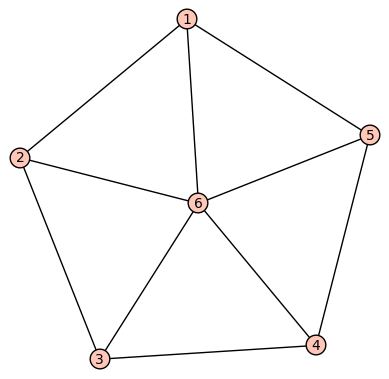
\includegraphics[width=0.5\textwidth]{odd_pyramid.png}
\end{figure}
Before producing the rewriting system, let us explain how the class constructor works. As mentioned above, if the parameter given to the constructor was a graph representing a triangulation, the QP will be automatically generated. If the flag \texttt{add\_zero\_rules} is marked as \texttt{False}, the \texttt{rewriting\_rules()} method will produce the set of usual rewriting rules (the ones associated to the grevlex order) and perform \hyperref[heuristic]{Heuristic \ref*{heuristic}} indefinitely until confluence is achieved. In order to test confluence, for every ambiguity we reduce both of its branches a maximum of \texttt{ambiguity\_depth} times and compare if both branches eventually resolve to the same element.

If \texttt{add\_zero\_rules} is set to \texttt{True}, the \textcolor{red}{not the same as implemented \texttt{zero\_rules()}} method will be executed before \texttt{rewriting\_rules()}. The \texttt{zero\_rules()} method performs the following heuristic:
\begin{heur} As we have seen in \hyperref[arbitrarily-long]{Observation \ref*{arbitrarily-long}},  any path that may be prolonged to a path of arbitrarily high length is zero. Reductions of the form $x\rightsquigarrow 0$ are highly desirable, since the ambiguities they generate are usually simple to resolve. Obviously, if $x=0$, then $yxz=0$ for all $y,z$, and so we are interested in finding only the shortest paths that reduce to zero. Therefore, we perform the following steps:
\begin{enumerate}
\item Let $n=2$.
\item Produce a list of all paths of length $n$.
\item Apply rewriting rules to each path until either they are irreducible or they are longer than \texttt{zero\_depth}.
\item If a path $x$ is equal to a path of length greater than \texttt{zero\_depth}, add the rewriting rule $x\rightsquigarrow 0$.
\item If no path was found to reduce to zero, increase $n$ by 1 and repeat steps 2 to 5.
\end{enumerate}
This may be formalized by a \textcolor{red}{pumping lemma argument} if we choose a high enough value for \texttt{zero\_depth}.
\end{heur}

We now generate the rewriting system associated to our pyramid:
\begin{lstlisting}
sage: odd_rs = Rewriting_System(odd_pyramid)
16 rules added.
3 rules added.
Total rules: 39
\end{lstlisting}
As we can see, the program had to enlarge the set of rules twice before achieving confluence. Let us examine the quiver and its associated potential, which both were generated automatically out of the triangulation:
\begin{lstlisting}
sage: odd_rs.quiver.show()
\end{lstlisting}
\begin{figure}[h]
\centering
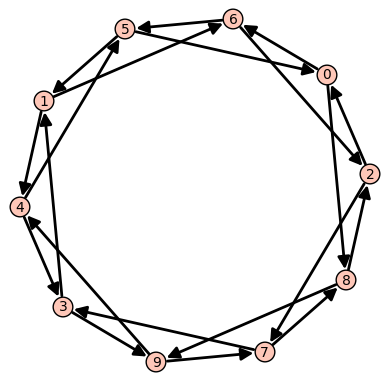
\includegraphics[width=0.5\textwidth]{odd_quiver.png}
\end{figure}
\begin{lstlisting}
sage: odd_rs.potential
[[3, 9, 7, 3],
 [8, 2, 7, 8],
 [0, 8, 9, 4, 5, 0],
 [4, 3, 1, 4],
 [5, 1, 6, 5],
 [2, 0, 6, 2],
 [0, 6, 5, 0],
 [0, 8, 2, 0],
 [8, 9, 7, 8],
 [9, 4, 3, 9],
 [5, 1, 4, 5],
 [6, 2, 7, 3, 1, 6]]
\end{lstlisting}
As the output shows, there are five 3-cycles coming from the triangular faces, a 5-cycle from the pentagonal face, five 3-cycles from punctures where three faces meet and another 5-cycle from the puncture corresponding to the apex of the pyramid.

\note{mostrar también las reglas de reescritura?}We may now compute the set of all irreducible paths up to a certain length. This is performed by just filtering the list of all paths. For instance, we may produce the list of all irreducible paths of length 4:
\begin{lstlisting}
sage: odd_rs.basis(5)[-1]
[[0, 8, 9, 4, 5],
 [0, 8, 9, 7, 3],
 [1, 6, 2, 7, 3],
 [1, 6, 5, 0, 8],
 [2, 7, 3, 1, 6],
 [2, 7, 8, 9, 4],
 [3, 1, 6, 2, 7],
 [3, 9, 4, 5, 0],
 [4, 5, 0, 8, 9],
 [4, 5, 1, 6, 2],
 [5, 0, 8, 9, 4],
 [5, 1, 6, 2, 7],
 [6, 2, 7, 3, 1],
 [6, 5, 0, 8, 9],
 [7, 3, 1, 6, 2],
 [7, 8, 9, 4, 5],
 [8, 9, 4, 5, 0],
 [8, 9, 7, 3, 1],
 [9, 4, 5, 0, 8],
 [9, 7, 3, 1, 6]]
\end{lstlisting}
The name of this method is \texttt{basis()} since the set of all irreducible paths of length $n$ is actually a basis of the homogeneous component of degree $n$ of the associated graded algebra, as we discussed in \hyperref[graded-alg]{Section \ref*{graded-alg}}. We may compute its Hilbert series up to a certain degree as well:
\begin{lstlisting}
sage: odd_rs.hilbert_series(15)
[10, 20, 20, 20, 20, 20, 20, 20, 20, 20, 20, 20, 20, 20, 20]
\end{lstlisting}
\note{incluir snippets para generar los otros poliedros}
\end{chapter}